\chapter{Asking Beverly Hills Billionaires How They Got Rich}

This chapter is built from a street lecture on wealth rather than from a blackboard lecture on theory. The lecturer begins with scale, celebrity, and access, then gradually discovers what can actually be transported from one fortune to another. The arithmetic is simple, but it is not incidental. It appears at the exact points where the lecture wants to separate appearance from mechanism: revenue from cash, income from preservation, and prestige from enough.

\section{Beverly Hills as a Wealth Field}

The lecture opens with a teaser montage. Its job is not yet to explain anything. It is there to establish magnitude: billionaires, dominant athletes, private events, and a promise that the richest people in Los Angeles may be stopped long enough to say how they built what they built. Only after this does the setting come into focus. Beverly Hills is presented as a dense field of wealth, a small geography in which money, influence, and visibility are unusually concentrated.

An early failed contact, partly buried under phone chatter, matters for the structure of the lecture even though it contributes almost no doctrine. It shows that access is not free. The method of the lecture is therefore not abstract instruction but repeated approach under friction: we ask, we are ignored, we ask again, and only then do we get a usable answer.

This is important because the lecture never begins from a balanced taxonomy of wealth. It begins from encounter. The order is practical: first find somebody who has actually crossed the boundary into very large money, then ask what number, habit, or decision survives compression.

\section{Scale, Debt, and the First Billionaire}

The first long interview establishes endpoint before origin. The woman first reports that she became a millionaire at twenty-eight. She then reminds the interviewer that he has not yet asked when she became a billionaire. The lecture uses this small comic beat to make a serious point: the scale we are dealing with is not local success but global scale.

The spoken numerical claims can be written compactly as
\begin{align}
N_{\text{companies}} &> 10,\\
Y_{6\text{mo}} &= \$80 \times 10^6.
\end{align}
The first number tells us that the fortune is diversified across many companies. The second gives the lecture one of its few hard monetary magnitudes.

\paragraph{Worked example.}
If we do nothing more than translate the six-month figure into a monthly equivalent, we obtain
\begin{align}
Y_{\text{month}} &\approx \frac{Y_{6\text{mo}}}{6}
= \frac{\$80 \times 10^6}{6}
\approx \$13.3 \times 10^6/\text{month}.
\end{align}
We should not overread this as a law of steady earnings. It is only the arithmetic of a reported burst. But the lecture wants the audience to feel the size of the claim, and this conversion helps.

Only after these endpoint numbers are on the table does the interview reverse into its starting wound. The initial condition is not inherited comfort but inherited liability:
\begin{equation}
D_0 = -\$3 \times 10^6.
\end{equation}
The lecturer is careful here. This was debt, not cash. In other words, the story begins not merely from zero but from a negative balance sheet.

From that point the interview extracts a first layer of doctrine. Ignorance is expensive. One must learn before drowning. One must stop spending energy trying to win approval from people who cannot even please themselves. The lecture then adds a second layer: formal education mattered here, not because it mechanically created wealth, but because it produced discipline. The woman insists on continued study, continued degrees, and continued learning. The lecture does not present education as a magic credential. It presents it as training in ordered effort.

\subsection{Question \& Answer}

The lecture now raises its sharpest local question.

What business number actually counts?

The answer is given against a false sequence. People aim first at sales. Then, if they have improved their vocabulary, they aim at profit. The interview rejects both stopping points.

\begin{definition}
Let \(R\) denote revenue, let \(\Pi\) denote nominal accounting profit, and let \(C_{\text{net}}\) denote the after-tax cash that can actually be taken out of the business and put into the owner's pocket.
\end{definition}

In the language of the interview, the operative target is not revenue and not even nominal profit:
\begin{equation}
\text{target} \neq R, \qquad \text{target} \neq \Pi, \qquad \text{target} = C_{\text{net}}.
\end{equation}
The reason is that profit can be corrupted by hidden weakness: bad debt, bad stock, and other balance-sheet contamination. A business may look impressive at the level of sales, and even respectable at the level of reported profit, while still failing the more brutal question: what can actually leave the business after tax?

\begin{figure}
\centering
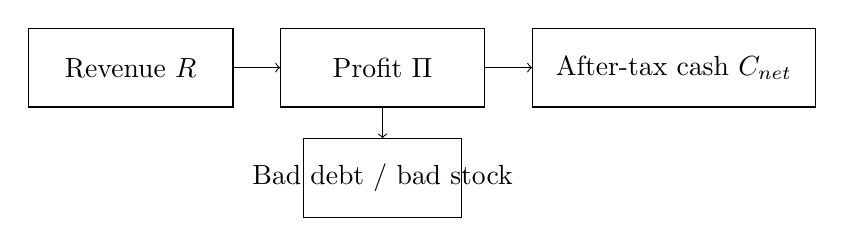
\begin{tikzpicture}[x=1cm,y=1cm]
\draw (0,0) rectangle (2.6,1) node[pos=.5] {Revenue $R$};
\draw (3.2,0) rectangle (5.8,1) node[pos=.5] {Profit $\Pi$};
\draw (6.4,0) rectangle (10.0,1) node[pos=.5] {After-tax cash $C_{\text{net}}$};
\draw[->] (2.6,.5) -- (3.2,.5);
\draw[->] (5.8,.5) -- (6.4,.5);
\draw (3.5,-1.4) rectangle (5.5,-.4) node[pos=.5] {Bad debt / bad stock};
\draw[->] (4.5,0) -- (4.5,-.4);
\end{tikzpicture}
\end{figure}

This diagram is a transcript-backed reconstruction, not a photographed board. Its function is simply to preserve the spoken distinction. The lecture is insisting on a cash waterfall. We start with scale, pass through the accounting mask, and ask what money is truly extractable.

\begin{remark}
The interview does not provide a full accounting identity. It gives a ranking of business quantities. The notation \(R\), \(\Pi\), and \(C_{\text{net}}\) is therefore a compact companion to the spoken point, not a claim about the lecturer's exact symbols.
\end{remark}

\section{Mentors, Mobility, and the Poverty Loop}

Having corrected the business metric, the lecture widens outward. Wealth is now described not only as a balance-sheet phenomenon but also as a social and geographical one. The advice is severe: if one wants to escape poverty, one should attach oneself to at least one rich person. The lecture's claim is that the wealthy do not merely possess capital; they also possess templates, examples, introductions, and sometimes startup money. The poor, by contrast, are described here as a gravity well.

This is a strong claim, and the lecture means it strongly. It is part social theory, part provocation, part motivational strike. What matters for the notes is the mechanism it proposes: mentorship changes the set of examples one lives inside.

The same pattern appears in the travel advice. Leaving one's hometown is not treated as ornament or lifestyle branding. It is treated as an economic change of coordinates. One crosses an ocean, leaves comfort, and is forced into new perception. In the interview's language, even one's neurons change.

\subsection{Question \& Answer}

Can we become rich while staying comfortable, local, and approved?

The answer given by the lecture is no, or at least not by the route it is describing here. Approval seeking wastes energy. Staying fixed preserves the scale of one's present world. Travel disrupts that scale.

A compact way to preserve the lecture's logic is
\begin{equation}
\text{movement} \to \text{discomfort} \to \text{exposure} \to \text{change of self and business horizon}.
\end{equation}
The line ``you're not a tree'' is humorous, but it contains the whole doctrine. Human capital is mobile. If one insists on sitting on a couch, then even that couch should at least be in Paris. The lecture is not arguing for tourism. It is arguing against the economics of fixed identity.

The final line of this segment deepens the same point. Things happen for you, not merely to you. In the lecture's rhythm, adversity is not erased; it is reclassified as preparation. This links back to the earlier inherited debt. The chapter's first major fortune does not begin from clean conditions. It begins from a deficit and then interprets difficulty as training rather than verdict.

\section{Communication as Economic Infrastructure}

The next interview changes the axis of analysis. We move from multi-company scale and cash extraction to communication itself as a productive asset. Dr. Forbes Riley is introduced first through recognition, then through numbers, and only after that through doctrine. She says she created one of the great fitness products on the planet, but insists that she is more than a business owner. She also masters the art of communication.

Again the lecture quickly condenses this into money:
\begin{align}
V_{\text{sales}} &> \$2.5 \times 10^9,\\
R_{\text{day}} &= \$1 \times 10^6/\text{day}.
\end{align}
These are not claims about net worth. They are claims about sales scale and sales velocity.

The conceptual move of the segment is even cleaner than the numbers. Pitching is defined functionally: it is the ability to get someone to say yes. The first yes matters because it opens the next door. A credit card, an agent, a meeting, a chance, an order, a distribution channel: the lecture treats all of these as children of the first yes.

We may preserve that mechanism schematically as
\begin{equation}
\text{communication} \to \text{persuasion} \to \text{yes} \to \text{access/opportunity}.
\end{equation}
In this section the lecture is not talking about communication as decoration. It is talking about it as leverage. The sentence ``if you can communicate what you want, you win'' is not meant poetically. It is a claim about control over entry points.

The segment becomes sharper when the interview is interrupted. Filming must stop; privacy must be protected; the event resists documentation. Instead of weakening the point, the interruption strengthens it. Dr. Forbes Riley answers with the rule ``don't ask for permission; ask for forgiveness'' and then gives the concrete example that justifies the rule. Unable to find an agent, she created a manager, created a company, and represented herself. The lecture's logic here is unmistakable: when the formal gate is closed, one may have to fabricate the missing institution.

A brief self-recap follows. The lecturer compresses the first two entrepreneurial interviews into one transferable thesis: the billionaires he has met all mastered attention. Whatever else we think of the promotional interlude that follows, structurally it does one useful thing. It interprets communication not as mere self-expression but as a scarce economic skill.

\section{Attention, Athletics, and Preservation}

The Miles Garrett segment asks whether the earlier lessons survive when wealth comes not from selling a product but from athletic dominance. The answer is largely yes, though the vocabulary shifts.

The interview first fixes scale through a lower bound rather than an exact figure. The interviewer climbs a numerical ladder, and Garrett keeps answering yes. The safe conclusion is therefore
\begin{equation}
Y_{\text{Miles}} > \$20 \times 10^6.
\end{equation}

\paragraph{A clean lower bound.}
The logic of this estimate is worth recording explicitly.
\begin{enumerate}
\item The interviewer asks whether the yearly amount is greater than \$10 million.
\item Garrett answers yes.
\item The interviewer raises the threshold to \$15 million.
\item Garrett answers yes again.
\item The interviewer raises the threshold once more to \$20 million.
\item Garrett again answers yes.
\item Therefore the transcript supports a lower bound, not an exact value: \(Y_{\text{Miles}} > \$20 \times 10^6\).
\end{enumerate}

The lecture then reverses, as it did earlier, from scale to origin. Garrett did not come from money. His motive is family, especially his grandmother. The interview now asks the natural second question: not how to make money, but how not to destroy it. Garrett's answer is brief but concrete. He names teams and renewable energy, adds part ownership in the Cavaliers, and says he wants ownership in a Premier League club. The lecture is therefore no longer about earnings flow alone. It is about converting high current income into durable claims on future enterprises.

The deepest line in this section is older than finance. Be all in or all out. One cannot do anything half-heartedly and expect greatness. This line functions here almost as an update rule for effort:
\begin{equation}
\text{greatness requires total commitment, not partial participation.}
\end{equation}
The notation is verbal because the lecture is verbal here. But the structure is exact. If one wants elite output, one must supply undivided effort.

The interview then ties money back to character. Garrett says he does not worry about haters. He gives glory to God. In the lecture's sequence, faith is not a decorative afterthought. It appears after money, after performance, and after preservation, as one more answer to the question of what keeps a person ordered when public scale has already arrived.

\section{Spend, Trust, and the Arithmetic of Enough}

The final movement of the lecture takes us to the Beverly Hills Hilton and a red-carpet setting. Even clothing becomes part of the method. The interviewer changes dress because access depends on fitting the local code. Once inside, the lecture acquires its cleanest lifestyle formula through Ken Ricci of Flexjet.

Before the formula comes company scale:
\begin{align}
N_{\text{planes}} &\approx 370,\\
N_{\text{employees}} &\approx 5000.
\end{align}
Then comes a softer but still important trait inventory: passion and fanatical attention to detail. Wealth, the lecture suggests, is not only large intention but also disciplined care for small asymmetries.

\subsection{Question \& Answer}

When are we actually rich?

This is the most explicit quantitative question in the lecture, and it receives the cleanest numerical answer.

\begin{definition}
Let \(S\) denote annual spend, the amount required to live the life one actually wishes to live. The interview's richness threshold is the heuristic
\begin{equation}
W^\ast = 25S,
\end{equation}
where \(W^\ast\) is the stock of wealth at which one counts as rich in this spend-relative sense.
\end{definition}

The lecture immediately supplies examples:
\begin{align}
S &= \$1000/\text{year}
\qquad \Longrightarrow \qquad
W^\ast = \$25{,}000,\\
S &= \$10 \times 10^6/\text{year}
\qquad \Longrightarrow \qquad
W^\ast = \$250 \times 10^6.
\end{align}
This is the chapter's strongest corrective to prestige thinking. The wrong question is ``Do I have ten million or twelve million?'' The right question is ``What does my life actually cost?'' Wealth is thus made relative to burn rate, not to headline vanity.

\begin{remark}
The factor \(25\) is presented in the interview as a rule of thumb. The notes should preserve it as a heuristic of spend-relative sufficiency, not as a universal theorem of finance.
\end{remark}

The lecture does not stop at the formula. It turns immediately to family and trust. Ricci argues that parents speak too easily about sex and too little about money, even though money is one of the major practical realities children must eventually steward. He then recalls a lesson from President Clinton: trust is built when one begins by disclosing a fault. The extrapolation to family life is direct. If children are to trust parents about money, money cannot remain one of the untouchable household secrets.

In this way the lecture performs one final turn. It begins from billion-dollar scale, passes through cash flow, persuasion, and spending heuristics, and ends with empathy. The last answer in the chapter is that success rests on thinking about others: employees, family, and the human memory of how one made people feel. Arithmetic survives to the end, but it no longer stands alone.

\section{Summary}

This lecture begins by hunting wealth in public and ends by extracting three durable rules. First, scale must be translated into the right variable: not revenue, not nominal profit, but after-tax cash that can really leave the business. Second, wealth is social and mobile: mentors, travel, communication, and attention all change what opportunities can even be seen. Third, enough has an arithmetic. If annual spend is \(S\), then the interview's operative threshold is \(W^\ast = 25S\). The chapter closes by joining that arithmetic to stewardship. Money is not only accumulated, sold, pitched, preserved, or spent. It is also disclosed, taught, and humanized.